\documentclass[conference]{IEEEtran}
\IEEEoverridecommandlockouts
% The preceding line is only needed to identify funding in the first footnote. If that is unneeded, please comment it out.
%Template version as of 6/27/2024

\usepackage{cite}
\usepackage{amsmath,amssymb,amsfonts}
\usepackage{algorithmic}
\usepackage{graphicx}
\usepackage{textcomp}
\usepackage{xcolor}
\usepackage{booktabs}
\def\BibTeX{{\rm B\kern-.05em{\sc i\kern-.025em b}\kern-.08em
    T\kern-.1667em\lower.7ex\hbox{E}\kern-.125emX}}

% Added manually:
\usepackage{tikz}
\usetikzlibrary{arrows.meta, positioning, fit}
\usepackage{hyperref}
    
\begin{document}

\title{Efficient Environment Exploration and 3D Reconstruction with Reinforcement Learning and Multiple View Geometry}

% 1\textsuperscript{st} % could be used for 1.
\author{\IEEEauthorblockN{Frank Zillmann}
\IEEEauthorblockA{\textit{Department of Computer Engineering} \\
\textit{Technical University of Munich (TUM)}\\
Munich, Germany \\
frank.zillmann@tum.de}
}

\maketitle

\begin{abstract}
Within this project the problem of autonomous 3D scene reconstruction is tackled through a combination of reinforcement learning and classical multi-view geometry techniques.
A simulated Franka Panda robot equipped with a wrist-mounted RGB-D camera explores a tabletop scene containing randomly placed primitive objects.
Depth observations are incrementally fused into a Truncated Signed Distance Field (TSDF) using either Open3D or NVIDIA nvblox, and the resulting reconstruction is compared against a ground-truth mesh at every step---using Chamfer distance or a voxel-wise TSDF error---to compute the reward signal.
The robot policy predicting the robot motion can use multiple observations in a modular structure, among them the previous trajectory using a Transformer or renderings and uncertainty data of the current reconstruction using Convolutional Neural Networks, and is trained with Proximal Policy Optimization (PPO).
Experiments show that the policy learns useful strategies such as moving upward and sweeping across the table, outperforming a simple scripted baseline. Challenges such as limited dependence on the configuration of objects on the table and the absence of long training runs due to memory leaks in the used libraries are discussed.
\end{abstract}

% \begin{IEEEkeywords}
% reinforcement learning, 3D reconstruction, active perception, TSDF, next-best-view planning
% \end{IEEEkeywords}

%======================================================================
\section{Introduction}

Reconstructing the 3D geometry of an environment from a sequence of depth or RGB-D images is a fundamental problem in robotics and computer vision.
Classical multi-view geometry pipelines such as Structure-from-Motion~\cite{schoenberger2016sfm} and volumetric fusion~\cite{curless1996volumetric} assume that images are collected by a human operator or a pre-programmed scanning trajectory.
In practice, the choice of viewpoints critically affects reconstruction quality: redundant views waste time while occluded regions remain unobserved.

% The \emph{next-best-view} (NBV) problem asks which camera pose should be selected next to maximally reduce reconstruction uncertainty.
% Traditional NBV methods rely on hand-crafted heuristics such as information gain or frontier-based exploration.
% Recently, learning-based approaches have emerged as a promising alternative, leveraging deep reinforcement learning (RL) to discover non-myopic viewpoint planning strategies directly from data~\cite{meli2025robotcellmodelingexploratory}.

Simultaneously, efficiently learning the 3D geometry of robot cells and workspaces to enable safe and effective operation is a critical capability for autonomous robots.
While other approaches try to tackle this problem through involving a human operator in the loop \cite{meli2025robotcellmodelingexploratory}, fully autonomous exploration and reconstruction is desirable for scalability and efficiency in frequently changing environments such as manufacturing floors or laboratories.

In this work, a modular framework was developed in which a simulated Franka Panda manipulator learns to move its wrist-mounted camera so as to maximize the reconstruction quality of a tabletop scene within a fixed episode horizon.
The main contributions are as follows:
\begin{itemize}
    \item A modular simulation environment built on robosuite~\cite{robosuite2020} including multiple reconstruction metrics and methods for reward shaping and computation of the ground-truth geometry.
    \item Integration of two volumetric reconstruction back-ends (Open3D~\cite{zhou2018open3d} and NVIDIA nvblox~\cite{nvblox}) with a common interface.
    \item A multi-input policy architecture that modularly fuses multiple spatial observation modalities (camera pose history, 2D images, 3D reconstruction uncertainty).
    \item A training pipeline using PPO that allows flexibly choosing the reconstruction policy, reconstruction metric, observations, and other hyperparameters via an environment wrapper with a Gymnasium interface.
\end{itemize}

\begin{figure}[h]
\centering
\includegraphics[width=\linewidth]{episode_overview.png}
\caption{Screenshot of an evaluation episode.}
\label{fig:episode_overview}
\end{figure}

%======================================================================
\section{Related Work}

\textbf{Volumetric 3D Reconstruction.}\quad
Curless and Levoy~\cite{curless1996volumetric} introduced TSDF-based volumetric fusion, which remains the dominant paradigm for real-time depth integration.
Open3D~\cite{zhou2018open3d} provides a widely used open-source implementation based on voxel block grids, while NVIDIA's nvblox accelerates integration and querying on GPUs.
Neural implicit representations~\cite{Liao_2024_WACV, Guo_2024_UNIKD, Younes_2024_SparseCraft} offer an alternative but are currently too slow for online RL training loops.

\textbf{Next-Best-View Planning.}\quad
Classical Next-Best-View Planning methods greedily select the next viewpoint that maximizes an information-theoretic criterion.
This work follows a similar motivation but focuses on techniques for learning the next-best-view using Reinforcement Learning specifically with a robot arm but without specializing on a specific reconstruction method or training on a shape dataset.

\textbf{Reinforcement Learning and Robot Simulation.}\quad
PPO~\cite{schulman2017proximalpolicyoptimizationalgorithms} is a widely used on-policy algorithm that provides stable training with clipped surrogate objectives.
Stable-Baselines3~\cite{stable-baselines3} offers a reliable PPO implementation and is used in this work.
The robosuite simulator~\cite{robosuite2020} provides standardized manipulation environments with MuJoCo~\cite{todorov2012mujoco} physics and has been extended in this project with a custom reconstruction task.

%======================================================================
\section{Methods}

The system is decomposed into three components (Fig.~\ref{fig:architecture}):
\begin{itemize}
    \item \textbf{Robot Environment:} The simulated environment in which the robot operates, including the computation of the 3D reconstruction errors and rewards.
    \item \textbf{Reconstruction Policy:} The method used to reconstruct the 3D environment from the robot's observations.
    \item \textbf{Robot Policy:} The reinforcement learning policy and its neural architecture that decides the robot's actions based on multiple observations.
\end{itemize}

From a reinforcement learning perspective, the combination of Robot Environment (\texttt{Reconstruct3D.py}) and Reconstruction Policy (\texttt{open3d\_reconstruction\_policy.py} or \texttt{nvblox\_reconstruction\_policy.py}) forms the total environment, while the Robot Policy is the agent that interacts with it.
This separation is reflected in the code, where \texttt{reconstruct3D\_gym\_wrapper.py} handles all interactions between the robot environment and the reconstruction policy and assembles the observations for the robot policy.

\begin{figure*}[t]
\centering
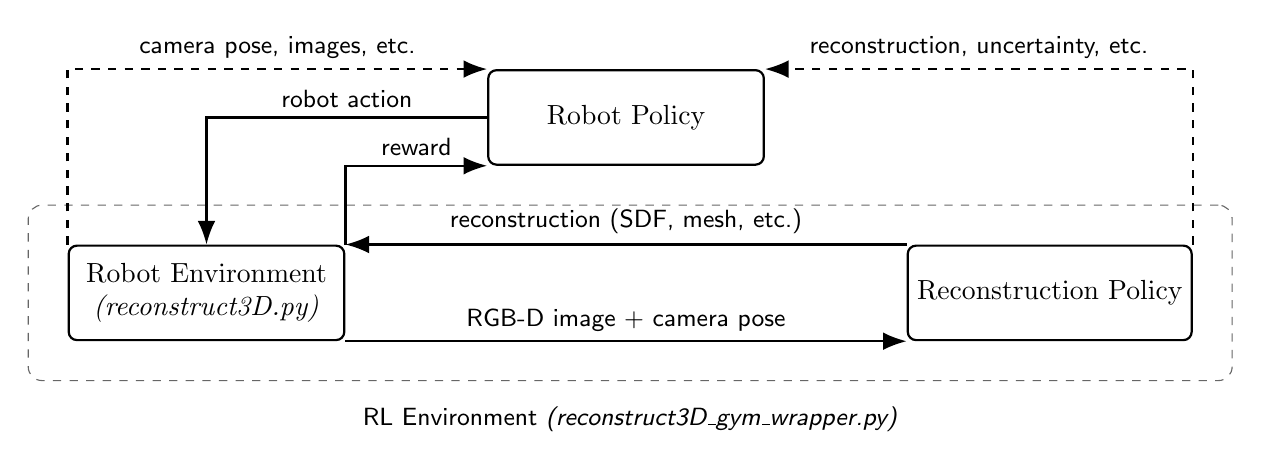
\begin{tikzpicture}[
  box/.style={draw, thick, rounded corners=3pt, minimum width=35mm, minimum height=12mm, align=center},
  arrow/.style={-{Latex[length=3mm]}, thick},
  dashedarrow/.style={-{Latex[length=3mm]}, thick, dashed},
  label/.style={font=\small\sffamily},
]

% --- Node placement (grid-like for zero clutter)
\node[box] (robot)                      {Robot Policy};
\node[box, below left=10mm and 18mm of robot]  (env)   {Robot Environment\\
\textit{(reconstruct3D.py)}};
\node[box, below right=10mm and 18mm of robot] (recon) {Reconstruction Policy};

% --- RL observation region
% \node[
%   draw=blue!60, dashed, rounded corners=5pt,
%   fit=(env)(recon),
%   inner sep=5mm,
% ] (group) {};

\node[
  draw=black!60, dashed, rounded corners=5pt,
  fit=(env)(recon),
  inner sep=5mm,
] (group) {};

\node[
  below=2mm of group,
  label,
  align=center,
  text width=80mm
] {
  RL Environment \textit{(reconstruct3D\_gym\_wrapper.py)}
};

% --- Arrows

\draw[arrow] (robot.west) -| node[label, near start, above]
  {robot action} (env.north);

\draw[arrow] (env.north east) |- node[label, near end, above]
  {reward} (robot.south west);

\draw[arrow] (env.south east) |- node[label, near end, above]
  {RGB-D image + camera pose} (recon.south west);

\draw[arrow] (recon.north west) |- node[label, near end, above]
  {reconstruction (SDF, mesh, etc.)} (env.north east);

% --- Arrows for observations

\draw[dashedarrow] (env.north west) |- node[label, near end, above]
  {camera pose, images, etc.} (robot.north west);

\draw[dashedarrow] (recon.north east) |-
  node[label, near end, above] {reconstruction, uncertainty, etc.} (robot.north east);

\end{tikzpicture}
\caption{System architecture. Solid arrows show the simulation loop; dashed arrows show observation flow to the RL agent. The wrapper encapsulates the environment and reconstruction module behind a standard Gymnasium interface.}
\label{fig:architecture}
\end{figure*}
%----------------------------------------------------------------------
\subsection{Robot Environment}

The environment is built on robosuite~\cite{robosuite2020} with MuJoCo physics.
A Franka Panda 7-DoF manipulator is placed in front of a table ($1.0 \times 1.0$\,m) on which 4 primitive objects (boxes and cylinders of randomized sizes in $[0.05, 0.2]$\,m) are placed at random positions and orientations at each episode reset.
The robot carries an RGB-D camera ($128 \times 128$\,pixels) on its end-effector (TCP).
The environment allows for further cameras such as frontview and birdview cameras, used for evaluation visualization and as additional observations for the policy.

\textbf{Action Space.}\quad
The robot is controlled via an Operational Space Controller (OSC\_POSE) that accepts 6-DoF delta commands $\mathbf{a} = [\Delta x, \Delta y, \Delta z, \Delta r_x, \Delta r_y, \Delta r_z] \in [-1, 1]^6$ in the global world coordinate frame.
These are scaled to position deltas of $\pm 0.05$\,m and orientation deltas of $\pm 0.25$\,rad per control step.
The control frequency is 4\,Hz and the episode horizon is 32 steps (8\,s of simulated time).

\textbf{Ground Truth.}\quad
At each episode reset, the ground-truth mesh of the static scene desired for reconstruction (table plate and primitive objects on it, no table legs, walls, etc.) is extracted from MuJoCo's collision geometry, and its axis-aligned bounding box (with 5\% padding) defines the bounding box where the ground truth SDF is computed.
For the voxel-wise TSDF metric, the ground-truth SDF is additionally computed on a $32^3$ grid via \texttt{mesh2sdf}~\cite{marian42_mesh_to_sdf}.

%----------------------------------------------------------------------
\subsection{Reconstruction Policy}

At every simulation step, the wrapper extracts the wrist camera's depth image, intrinsic matrix, and extrinsic pose, and passes them to the reconstruction policy's \texttt{add\_obs} method.
Two reconstruction policies are supported:

\textbf{Open3D TSDF}~\cite{zhou2018open3d}: Uses the tensor-based \texttt{VoxelBlockGrid} API for depth-only integration with configurable voxel size, truncation distance, and maximum depth.
Mesh extraction is performed via marching cubes.
This back-end runs on CPU or GPU and requires no NVIDIA-specific drivers.
It only allows querying the reconstructed mesh, so the reward is computed via Chamfer distance to the ground-truth mesh.

\textbf{NVIDIA nvblox}~\cite{nvblox}: Provides GPU-accelerated TSDF integration in a similar manner to Open3D but requires an NVIDIA GPU and CUDA drivers.
Beyond mesh extraction, nvblox supports querying the TSDF and observation weights on a dense grid, which enables the voxel-wise TSDF error metric and weight-grid observations.

Both back-ends share a common interface (\texttt{BaseReconstructionPolicy}) with \texttt{add\_obs}, \texttt{reconstruct}, and \texttt{reset} methods, making it easy to switch between them via the configuration file without changing the training code and to add new reconstruction methods.
Default parameters are a voxel size of 0.01\,m, a truncation distance of 0.04\,m, and a maximum integration depth of 1.0\,m.

%----------------------------------------------------------------------
\subsection{Reconstruction Metrics and Reward Function}
\label{sec:reward}

Two error metrics quantify the deviation of the current reconstruction from the ground truth:

\textbf{Chamfer Distance (CD).}\quad
10\,000 points are sampled uniformly from both the reconstructed and ground-truth mesh surfaces via area-weighted barycentric sampling.
KD-trees are used for nearest-neighbor queries, and the metric is the symmetric mean $L_1$ instead of $L_2$ to reduce sensitivity to outliers, e.g.,\ small floating artifacts in the reconstruction.
\begin{equation}
    \mathrm{CD} = \frac{1}{2}\!\left(\frac{1}{N}\!\sum_{i=1}^{N}\!\min_{\mathbf{q}}\|\mathbf{p}_i - \mathbf{q}\|_1 + \frac{1}{N}\!\sum_{j=1}^{N}\!\min_{\mathbf{p}}\|\mathbf{q}_j - \mathbf{p}\|_1\right)
\end{equation}
where $\{\mathbf{p}_i\}$ and $\{\mathbf{q}_j\}$ are the sampled point sets.

\textbf{Voxel-wise TSDF Error.}\quad
The reconstructed TSDF is queried on the same $32^3$ grid as the ground truth.
The error has two components: (i)~the mean $L_1$ distance between observed TSDF values and the ground-truth SDF, and (ii)~a missing-voxel penalty equal to the fraction of near-surface voxels (ground-truth $|\text{SDF}| < 0.5 \cdot d_\text{trunc}$) that remain unobserved.
Voxels below $z_\text{table\_surface} - 0.5 \cdot d_\text{trunc}$ are excluded to avoid penalizing physically inaccessible regions beneath the table.

\textbf{Reward Shaping.}\quad
Two modes translate the error $e_t$ into a per-step reward:
\begin{itemize}
    \item \emph{Exponential}: $r_t = s \cdot \exp(-e_t / c)$, where $s=1.0$ is a scale and $c$ the characteristic error. This directly translates lower error into higher reward but also provides a positive signal for actions which preserve a current good reconstruction.
    \item \emph{Delta}: $r_t = s \cdot (e_{t-1} - e_t) / c$, which directly rewards error reduction at each step. Here $c=\frac{1}{\text{horizon}}$ was chosen as this would be the improvement if the error smoothly went from 1 to 0 over the whole episode. This provides a clearer learning signal for the policy to focus on actions that improve the reconstruction, but is noisier due to the dependence on the previous step's error.
\end{itemize}
A classic action penalty $\lambda \cdot \overline{|\mathbf{a}_t|}$ with $\lambda = 0.1$ discourages unnecessarily large motions.

%----------------------------------------------------------------------
\subsection{Robot Policy Architecture}
\label{sec:policy}

The policy uses a \emph{MultiInputPolicy} (Stable-Baselines3~\cite{stable-baselines3}) with a modular feature extraction front-end (\texttt{CombinedExtractor}) that fuses information from multiple observation modalities.
Each sub-extractor processes a different observation key and produces a fixed-dimensional feature vector; the concatenated result is projected through a linear layer to a 256-dimensional combined representation, which is then fed into the policy and value network heads (two hidden layers of 256 units each).

The following sub-extractors are used:

\textbf{Camera Pose History (Transformer).}\quad
The sequence of 7-DoF camera poses (position + quaternion) collected during the episode is processed by a small Transformer encoder (1~layer, 4~heads, $d_\text{model}=64$, feed-forward dimension~256, maximum 32~steps).
Positional embeddings are added, zero-padded future steps are masked, and the output is mean-pooled over valid time steps to produce a 64-dimensional feature vector (56\,704 parameters).
This allows the policy to reason about where the camera has already been, avoiding redundant revisits.

\textbf{Image Features (CNN).}\quad
A birdview RGB image (3~channels) from a fixed overhead camera and a grayscale rendering of the current reconstruction mesh (1~channel) are concatenated channel-wise (4~input channels) and processed by a three-layer CNN (stride-2 convolutions with batch normalization, followed by adaptive average pooling), yielding a 128-dimensional feature vector (56\,848 parameters).
Images are resized to $64 \times 64$ in the forward pass. Furthermore, the user can choose to use only the RGB image, only the mesh rendering, neither, or both as input to the policy.

\textbf{Weight Grid (3D-CNN).}\quad
When using nvblox, the per-voxel observation weight grid ($32^3$, indicating how often each voxel has been observed) is processed by a three-layer 3D-CNN, producing a 128-dimensional feature vector (50\,560 parameters).
Weights are log-scaled ($\ln(1+w)$) before passing through the network.
This provides the policy with explicit spatial information about which parts of the scene lack observations.

The three sub-extractor outputs (dimensions 64, 128, 128) are concatenated into a 320-dimensional vector and projected to a 256-dimensional combined representation through a linear layer.
The entire feature extraction front-end comprises 246\,288 trainable parameters.

\begin{figure}[h]
\centering
\includegraphics[width=\linewidth]{robot_policy_architecture.png}
\caption{Robot policy architecture.}
\label{fig:policy_architecture}
\end{figure}

%----------------------------------------------------------------------
\subsection{Training}

Training uses PPO mostly with default parameters. The discount factor $\gamma$ was set to 0.98 because of the rather short horizon, and the entropy coefficient was set to 0.01 to encourage exploration.
Four parallel environment instances are used for data collection, and a separate evaluation environment with deterministic seeding logs images, meshes, and rewards every 50\,000 steps.
Training was conducted on a CPU-only laptop (Open3D, Chamfer distance metric) and on a Google Cloud VM with an NVIDIA T4 GPU (nvblox back-end, voxel-wise TSDF error). Many of the discussed features were implemented iteratively based on previous results over the course of the project, so a direct comparison of all training curves is not possible.

% \begin{table}[t]
% \centering
% \caption{PPO Hyperparameters}
% \label{tab:hyperparams}
% \begin{tabular}{@{}ll@{}}
% \toprule
% Parameter & Value \\
% \midrule
% Horizon (steps/episode) & 32 \\
% Control frequency & 4\,Hz \\
% Parallel environments & 4 \\
% Rollout length ($n_\text{steps}$) & 512 per env \\
% Minibatch size & 128 \\
% Epochs per update & 5 \\
% Learning rate & $3 \times 10^{-4}$ \\
% Discount factor $\gamma$ & 0.98 \\
% GAE $\lambda$ & 0.95 \\
% Clip range & 0.2 \\
% Entropy coefficient & 0.01 \\
% Total timesteps & $2 \times 10^6$ \\
% Reward mode & delta \\
% Action penalty $\lambda$ & 0.1 \\
% Characteristic error $c$ & $1/32$ \\
% Camera resolution & $128 \times 128$ \\
% SDF grid resolution & $32^3$ \\
% \bottomrule
% \end{tabular}
% \end{table}

%======================================================================
\section{Results and Discussion}
%======================================================================

\subsection{Training Challenges}
A major problem for the effective training and evaluation of the described approaches were memory leaks in the used libraries, which prevented long training runs.
While an initial segmentation fault caused by the rendering of the current reconstruction could be fixed by switching from Open3D's visualizer to a custom off-screen renderer, a leak in nvblox caused the GPU memory usage to grow over time until the process was killed after several hours of training.
Therefore, the final training run was limited to 250\,000 steps, which is relatively short for a complex RL problem and may have prevented the policy from fully converging.
Furthermore, interesting ablation studies such as the effect of different reward shaping methods, observation modalities, or reconstruction back-ends could not be conducted due to the difficulty of running multiple long training runs.

\subsection{Policy Performance and Iterative Improvements}
The first runs showed the robot strongly jiggling the camera and frequently moving it away from the scene, which could be largely fixed through the addition of the action penalty and the delta-based reward shaping.

Early experiments used an exponential reward $r_t \propto \exp(-e_t/c)$ that provides positive feedback at every step.
While stable, this signal was found to plateau quickly because the absolute error level provides less information about the \emph{marginal} value of each action.
Switching to the delta formulation $r_t \propto (e_{t-1} - e_t)$ provided a direct signal for error reduction and improved learning speed.

The Chamfer distance is a natural geometry-based metric but has non-trivial computational cost ($\sim$50\,ms per evaluation for 10\,000 sample points) and variance/noise due to stochastic point sampling.
The voxel-wise TSDF error is deterministic and provides separate signals for accuracy (observed-voxel error) and coverage (missing-voxel penalty), but requires the nvblox back-end to query the TSDF on a dense grid.

Adding the camera pose history via the Transformer encoder improved performance, which is expected as the agent can better avoid revisiting the same viewpoints but it might also have led to less dependence on the configuration of objects on the table, as the policy can learn to simply follow a fixed sweeping trajectory without needing to adapt to the specific scene.
Further ablation studies would be needed to investigate this hypothesis.

The pre-final run (Fig.~\ref{fig:training_curve}) showed a steady increase in evaluation reward and even slightly outperformed the scripted baseline, which moves over the table in a fixed trajectory and yields an average reward of $19.86 \pm 4.3$.
However, this policy often steered the robot to the side and below the table at the end of the episode, likely because voxels below the table surface could sometimes be observed from these positions, or because the reward signal becomes very noisy when the reconstruction is already good.
To address this, the below-table voxels were excluded from the reward computation. The final training run with this change and the addition of the birdview image as input no longer shows this behavior, confirming the hypothesis.

\begin{figure}[h]
\centering
\includegraphics[width=\linewidth]{eval_rewards.png}
\caption{Evaluation reward curves of final run (light blue) and longer pre-final run (dark blue) without birdview image and below-table voxel exclusion.}
\label{fig:training_curve}
\end{figure}

%======================================================================
\section{Conclusion}

A modular framework for RL-based active 3D reconstruction was developed, combining robosuite simulation, TSDF-based volumetric fusion (Open3D / nvblox), and a multi-modal PPO policy.
Delta reward shaping and pose-history observations proved most impactful; the learned policy slightly outperforms a scripted baseline despite limited long training runs and ablation studies by nvblox memory leaks.

\bibliographystyle{IEEEtran}
\bibliography{references}

\end{document}
